\chapter{Project Management}
\label{ch:project_management}

Appropriate project management is key to any projects success. Project management provides the core work flow and stages for a project. Providing a structure to work against to ensure goals are achieved, with progress tracked and checked. Below the Methodology, Timetable, Risk Management and Ethical, Legal, Social and Professional Issues for this project are discussed.

\section{Methodology}
The project followed an Agile \cite{atlassian_2022_what} approach, with a few plan driven aspects. Within this approach a backlog was generated using Notion \cite{notionlabs_2023_your} as a to-do list as seen in Figure \ref{fig:notion}. This to-do structure permitted the ability to create sub tasks, as indented lines, such that sub tasks could be completed independently of the parent task.

\begin{figure}
    \centering
    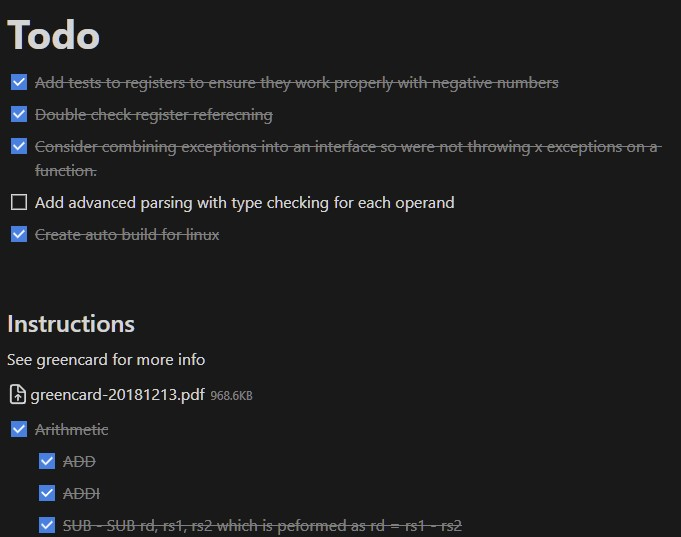
\includegraphics[width=0.8\textwidth]{dissertation/DATA/notion-todo.jpg}
    \caption{Backlog creates as a to-do list in Notion}
    \label{fig:notion}
\end{figure}

It may of been more appropriate to utilise the backlog within Github since it was being used for version control and could be tightly integrated. However, the simpler approach of using Notion was chosen as it was simpler to implement, modify and use, compared to creating lots of individual tasks on GitHub.

Only a handful of plan driven aspects existed, mainly being the overarching concepts of splitting the project into 3 core parts being the Emulator, Visualisation and eventually a module system, with a repetitive agile approach followed within each concept. In this case each individual element was continuously developed in increments with a consumable product available during the development cycle for testing and use.

A notable part of the agile approach was applying our ability to re-plan and re-design mid implementation. For example with the switch to percentages for animation, which required a new plan and design for the system. Another bigger example being the decision to implement the module system, which required mid project planning to identify how it would effectively work and integrate, followed by its individual design and implementation.

These major changes wouldn't of been as feasible if we had followed say a Waterfall methodology \cite{ganttchartsoftware_2023_waterfall}. This would of required restarting the core methodology loop, in order to make these changes as waterfall focuses on linear progress with a physical product available at the end of the development, whereas agile permits a quicker production of a viable product

\section{Timetable}
The project followed a weekly timetable split into 4 sections: Term 1, Term 2, Christmas and Easter as seen in Figures \ref{fig:tt_t1}, \ref{fig:tt_t2}, \ref{fig:tt_christmas} and \ref{fig:tt_easter} in Appendix \ref{app:timetable} respectively.

The timetables incorporate a weekly task, promoting a continuous linear flow of progress, with included breaks and catch-up weeks to ensure that delays were accounted for, and to ensure that burnout delays could be accommodated for. 

This timetable was followed mostly, with a few deviations including starting the next weeks content earlier, or delaying work into another week due to a higher course load. However, due to the efficient planning of the timetable, it proved useful for ensure productive use of time. It was also decided to plan the Christmas and Easter breaks to ensure work on the project continued, whilst allowing for more free time within these periods to relax and refresh.

A few alteration were made to the timetable towards the end. These included the removal of a scheduled holiday break, and the addition of the user feedback section. Further the allocation of time for the presentation was massively over-judged, allocating 5 weeks. Instead approximately 3 weeks were assigned to produce the slides, create the script, practice and finally present.

\section{Risk Management}
The project has been mainly risk free. The only main risk considered was the failure to produce a minimal viable product via the end of the Christmas break. However, this risk was quickly dismissed with a minimal viable produce ready post Christmas.

The only additional risk to consider was the possible loss of the code base due to unforeseeable circumstances. However, via the use of version control with \cite{github_2013_build} and Git \cite{git_2022_git}, as well as creating additional remote copies on the department system and zipped backup on google drive. The possibility of complete code loss has been made negligible, thus dismissing this risk.

\section{Ethical, Legal, Social and Professional Issues}
As a software development project very few Ethical, Legal, Social or Professional issues are present. No social or ethical issues exist, as no personal data has been collected or processed, and neither does the project cover any problematic content or areas of society.

There are a few considerations for legal and professional issues however, which are discussed below.

\subsection{Legal}
Java is not always free to use, dependent on the distribution used and its respective licence. In this respect Java is free to use for users, but may incur a cost for developers depending if they make use of additional paid options.

Thankfully, the project makes no use of paid features, and further makes use of the OpenJDK 19 \cite{oraclecorporation_2022_openjdk} distribution which has much fairer and lax rights usage compared to the OracleJDK and is commonly used for open-source projects.

Another consideration is the storage of user feedback data. Whilst no personal information was collected, it is still important to follow the General Data Protection Act \cite{theeuropeanparliamentandthecounciloftheeuropeanunion_2016_regulation} to ensure collected data is appropriately used, stored and then destroyed, with a notice to users visible. 

By using Google Forms, the collected data is only visible to the project, and can be easily destroyed, with the ability to easily display a GDPR notice on the form itself.

\subsection{Professional}
In a professional capacity, the project will need to ensure that standard principles are followed and maintained. Such as professional commenting and producing maintainable code. Further, ensuring that the resulting simulator is produced to a high standard, with no unnecessary gimmicks or alterations that may deter usage.
